% Tento soubor nahraďte vlastním souborem s obsahem práce.
%=========================================================================
% Autoři: Michal Bidlo, Bohuslav Křena, Jaroslav Dytrych, Petr Veigend a Adam Herout 2019
\chapter{Úvod}



\chapter{Teoretická část}

\section{Vlastnosti písania}

TODO
V tejto časti popíšem aké dáta chceme merať z písma.

\section{Existující technologie}

\subsection*{Livescribe 3}

Livescribe 3 je určené na písanie poznámok. Toto pero využíva Bluetooth v4.0 na spojenie s mobilným zariadením, do ktorého následne odosiela dáta o pohybe. Systém tieto dáta v reálnom čase prevádza do písaného textu, pričom je možné použiť aj funkciu konvertovania písaného textu do tlačenej podoby. Na záznam využíva infračervenú kameru, ktorá sa nachádza na spodnej časti pera pod hrotom tuhy. Okrem písma zaznamenáva aj zvuk a tak písmo doplňuje ďalší kontext. Veľkosťou je sa jedná o pomerne kompaktné zariadenie - 162x14.9 mm a hmotnosťou 34 gramov.\newline

\textbf{Hodnotenie:}
\begin{description}
	\item[+]{kompaktnosť}
	\item[+]{presnosť}
	\item[+]{nevyžaduje kalibráciu}
	\item[-]{infračervená kamera je príliš veľká, aby si ju používateľ nevšimol}
\end{description}

\subsection*{iskn Slate 2+}

Slate 2+ od firmy iskn využíva magnetický prstenec a špeciálnu podložku, v ktorej sa nachádza 32 magnetometrov (senzorov na meranie zmien magnetického poľa). Podložka komunikuje s aplikáciou v mobilnom zariadení alebo počítači pomocou Bluetooth LE v5.0 a v reálnom čase tieto dáta zobrazuje. Výsledok je veľmi presný, no vyžaduje presnú kalibráciu. Kalibrácia sa vykonáva tak, že sa na podložke stisne drží špeciálne tlačidlo a potom stačí vziať pero/ceruzku s prtencom a priložiť jej hrot kolmo na podložku. Následne stačí pustiť tlačidlo a všetko je nakalibrované. Ak sa kalibrácia nevykoná správne ceruzka nebude presnám \newline

\begin{figure}[hbt]
	\centering
	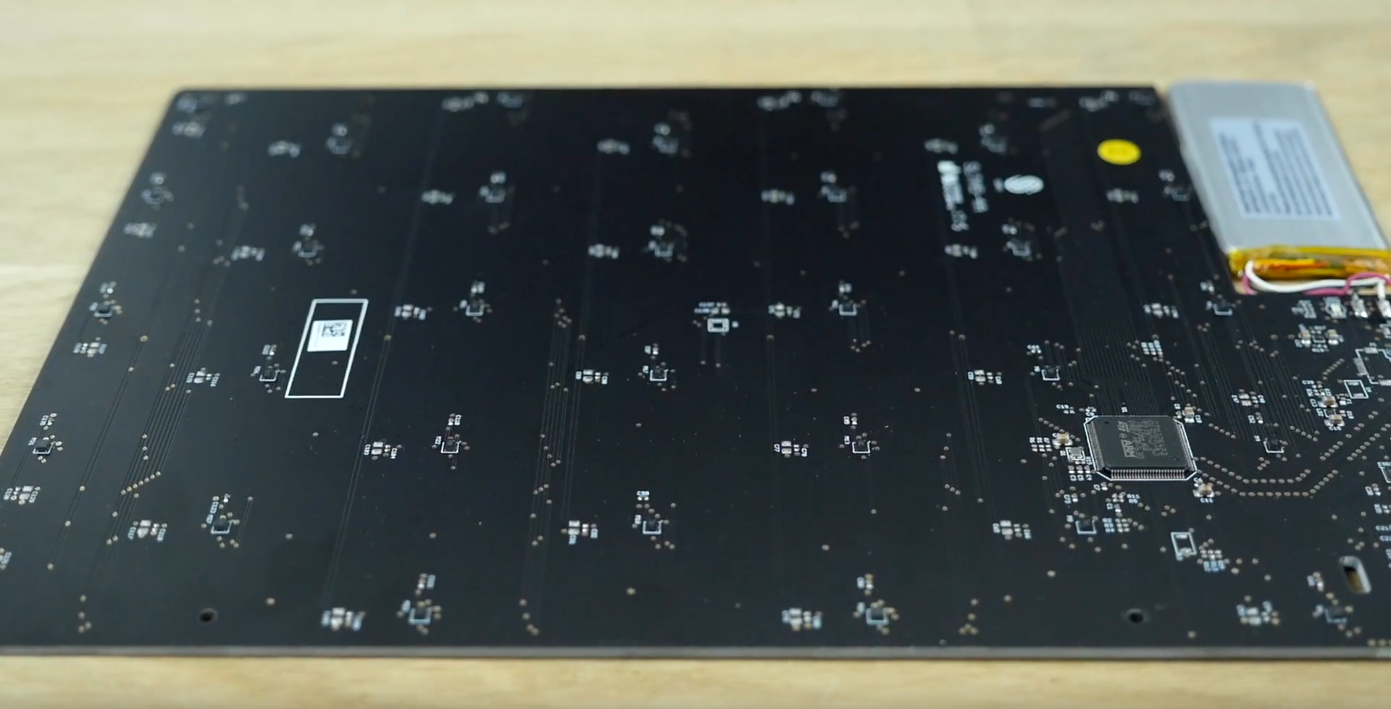
\includegraphics[width=0.5\textwidth]{obrazky-figures/isknBoard.png}
	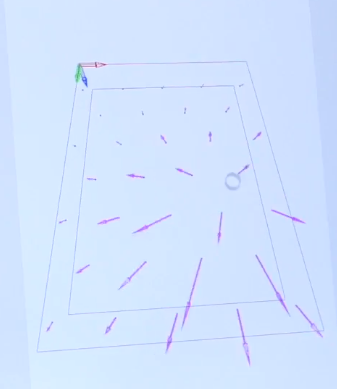
\includegraphics[width=0.3\textwidth]{obrazky-figures/isknMagneticfield.png}
	\caption{Board with sensors (left) and detected field (right)}
	\label{piezoPen1997}
\end{figure}
%isknMagneticfield
\textbf{Hodnotenie:}
\begin{description}
	\item[+]{nezáleží na použitom pere}
	\item[+]{písať sa môže čímkoľvek}
	\item[-]{vyžaduje podložku}
	\item[-]{kalibrácia}
\end{description}

\subsection*{Stylus}

Stylus sa používa na písanie na dotykové plochy. Aktuálne asi najsofistikovanejším je Apple Pencil. Radí sa mezdi aktívne stylusy\cite{HarleyJonahA2013As}. Používa dva trojosé gyroskopy rozmiestnené v rôznych častiach pera. Hrot pera funguje ako tlakový senzor a taktiež ako anténa, ktorá vysiela nízkofrekvenčné (dlhé) vlny a tie sú detekované senzorovou vrstvou pod displejom. Spojenie s iPadom zabezpečuje Bluetooth 4.1\cite{ApplePencilForum}. Intel v roku 2014 predpovedal, že aktívne stylusy nebudú také úspešné ako pasívne z dôvodu vysokej ceny a náročnosti vývoja takej technológie\cite{IntelDisp}. No ako môžeme vidieť, táto technológia nakoniec prerazila.\newline

\textbf{Hodnotenie:}
\begin{description}
	\item[+]{vysoká presnosť}
	\item[+]{realtime}
	\item[+]{nie je potrebná kalibrácia}
	\item[-]{náročnosť a komplexnosť vývoja}
	\item[-]{vyžaduje displej ako špeciálnu podložku}
	\item[-]{vysoká cena (keď rátame aj HW + displej a proprietárny software)}
	\item[-]{nefunguje so všetkými displejmi}
\end{description}

\subsection*{Návrh pera z roku 1977}

Jedná sa o pero so špeciálnou tuhou, ktorá má na sebe dva analógové piezoelektrické biomorfné senzory umiestnené v 90\degree~uhle k sebe navzájom. Podľa toho akou silou pôsobíme na hrot dokáže zaznamenať pohyb vďaka piezoeelktrickým javom.\cite{EernisseE}

\begin{figure}[hbt]
	\centering
	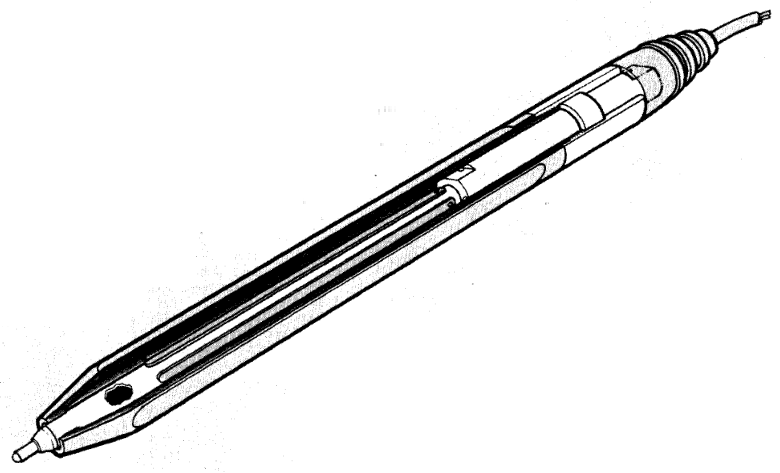
\includegraphics[width=0.3\textwidth]{obrazky-figures/piezoPen1997.png}
	\caption{Piezoelektrické pero}
	\label{piezoPen1997}
\end{figure}

Všetky tieto riešenia sa v praxi bežne používajú (okrem riešenia z roku 1977). Každý z týchto produktov má svoje použitie a podľa neho má aj prispôsobené použité technológie. V tejto práci si vyberiem parametre, ktoré budú spĺňať zadanie a navrhnem ďalšie rozšírenia. 

\chapter{Návrh řešení}

Cieľom tejto práce je vytvoriť pero so skrytými senzormi, ktoré budú snímať dynamické vlastnosti písma. 

\section{Výber komponent}

V tejto časti sa budem venovať výberu komponent a samotnému návrhu pera so senzormi.

\subsection*{Tlakový senzor}

Interlink Electronics FSR® 400 je malý a lacný tlakový odporový senzor. Bez záťaže sa správa ako nekonečný odpor a s použitím sily na jeho povrch sa jeho odpor znižuje. Citlivosť a~maximálna záťaž je nastavená na interakciu s ľuďmi. \cite{fsr400}
V kombinácii s 10K Ohm rezistorom a zapojením na analógový pin dáva najširí interval hodnôt.

\[
V_{OUT} = \frac{V_{IN} R_M} {R_M + R_{FSR}}
\]
\begin{figure}[hbt]
	\centering
	\includegraphics[width=0.7\textwidth]{obrazky-figures/.png}
	\caption{}
	\label{}
\end{figure}


\subsection*{Akcelerometer a akcelerometer}

Rozhodol som sa použiť modul GY-521, ktorý kombinuje obidva senzory na jednom čipe. Akcelerometre typu MEMS trpia zvýšenou hladinou šumu\cite{PawlusJan2019Zpns}, ako som sa aj ja presvedčil. Zatiaľ som mal k dispozícii len jeden modul preto som zatiaľ neotestoval použitie dvoch modulov a priemerovanie nameraných hodnôt. Ako alternatívu teraz čakám na ďalšie dva senzory DFROBOT SEN0253\cite{PohybovySenzor}, na ktorých vyskúšam priemerovanie a rôzne rozmiestnenie na pere.

\subsection*{SD karta}

Výber padol na adaptér microSD kariet DFROBOT DFR0229 kvôli jeho veľkosti a jednoduchému pripojeniu. Ako úložisko používam MicroSD kartu veľkosti 2GB. 

\subsection*{Mikrokontrolér}

Na začiatku som si vybral vývojovú dosku Arduino Nano kvôli jej jednoduchému použitiu a programovaniu. 
Počiatočné experimenty však ukázaly, že táto doska nie je vhodná, pretože jej ADC (analógovo digitálny prevodník) je príliš pomalý pri spracovávaní z viacerých senzorov. Mikrokontrolér dokázal spracovať\footnote{prečítať aktuálnu hodnotu z výstupu a zapísať ju do pamäte FLASH na SD karte} len asi 100 hodnôt za sekundu, čo je v mojom prípade málo, keže jeden podpis trvá približne do dvoch sekúnd.

Teraz som začal hľadať iný mikrokontrolér a vyskúšam vývojovú dosku ARMSTM32F103C8T6 \cite{ArduinoARM}. Tiež budem kontaktovať pána Ing. Václava Šimeka, ktorý mi hádam poradí ďalej.


\section{Návrh pera}

\subsection*{Uchytenie tlakových senzorov}

\begin{figure}[hbt]
	\centering
	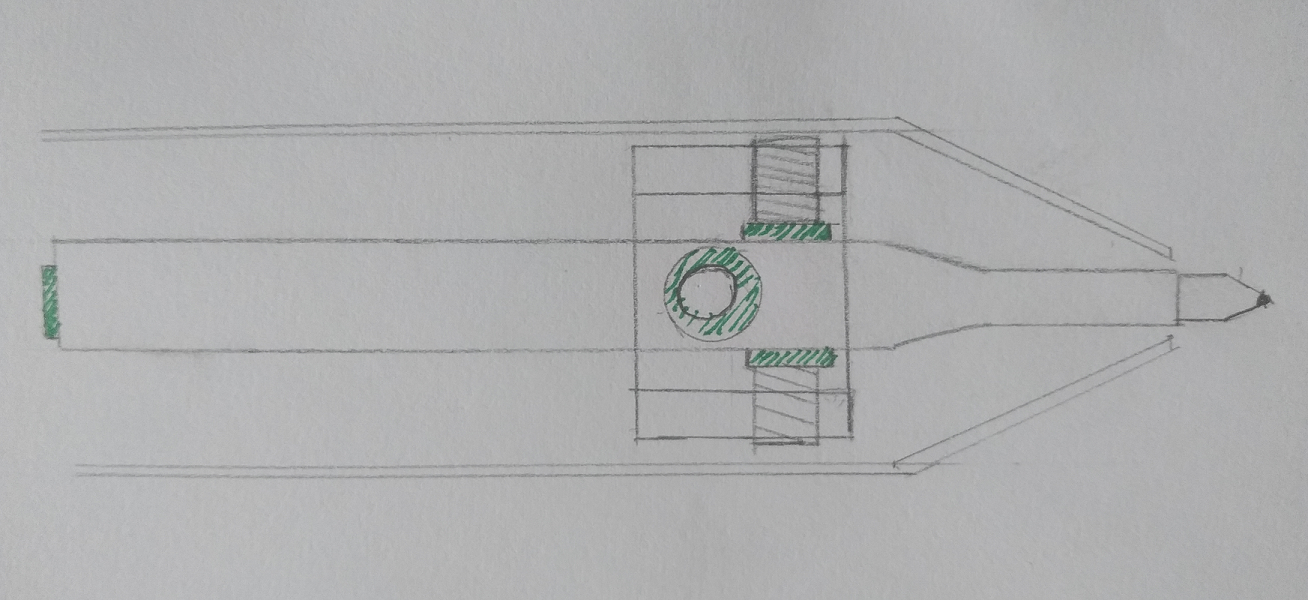
\includegraphics[width=0.7\textwidth]{obrazky-figures/umiestnenie_tlakovych_senzorov.png}
	\caption{Návrh uchytenia tuhy}
	\label{piezoPen1997}
\end{figure}

\begin{figure}[hbt]
	\centering
	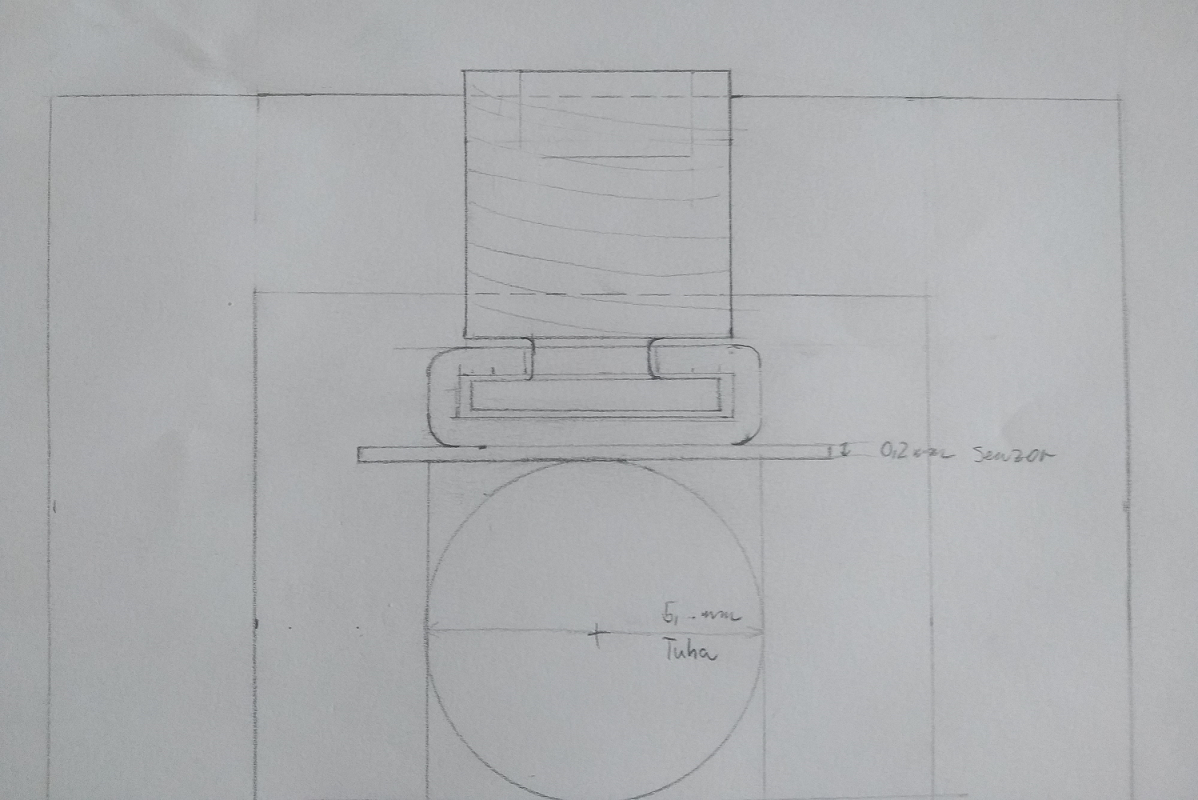
\includegraphics[width=0.7\textwidth]{obrazky-figures/uchytenie.png}
	\caption{Návrh uchytenia tlakového senzora}
	\label{piezoPen1997}
\end{figure}

\section{Nepoužité komponenty}

V tejto časti v skratke popíšem, ktoré súčiastky by sa mohli použiť v ďaľích prototypoch.

Mikrofón by sa mohol použiť ako senzor pre zachytenie širšieho kontextu, podobne ako to má Livescribe 3. Vedeli by sme potom k čomu sa písaný text viaže alebo aký dokument sa podpisuje. 

Ak by sme chceli merať ďalšie biometrické dáta mohli by sme použiť merač tepu na miestach kde sa človek dotýka pera. Ak bude osoba písať dlhší text vedeli by sme zistiť nakoľko je nervózna. 

Použitie bezdrôtového pripojenia, napr. BLE (Bluetooth Low Energy) by uľahčilo získavanie dát z pera, keďže ak sa chceme dostať k informáciám na SD karte musíme pero rozobrať. Toto riešnie by mohlo aj zmenšiť rozmery pera.

\chapter{Realizace řešení}

\section{Experimenty}

\subsection*{Testovanie súčiatok}

\begin{figure}[hbt]
	\centering
	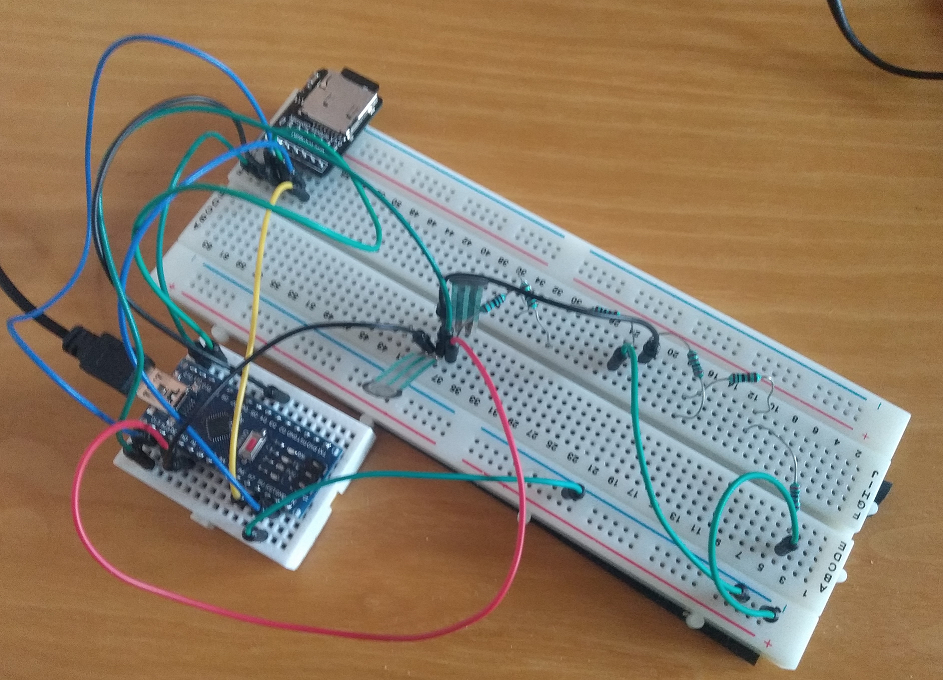
\includegraphics[width=0.5\textwidth]{obrazky-figures/FSRtestSD.png}
	\caption{Ukladanie dát na pamäťovú kartu}
	\label{Experiment1}
\end{figure}

\section{vyhodnocení výsledů}

\chapter{Závěr}

\label{zaver}

%===============================================================================
